\section{企業におけるアジャイルソフトウェア開発の実践}

本節では企業がどのようなツールを用いてアジャイルソフトウェア開発を展開しているかの具体例について述べる。

昨今の企業のインターネットサービス開発では、全体像としては企業やプロジェクトによってことなるが以下\ref{fig:dev_env}のような環境を用意する。開発用のコンピューターから、プログラムの変更をコードホスティングサーバーに送信すると、そのイベントを受け取った継続的インテグレーションツールが自動的に必要な手続きを踏み、検証環境にプログラムを展開する。検証環境で実際にプログラムに問題が無いことを確認した後、コードホスティングサーバーから本番環境への適用が行われる。

\begin{figure}[H]
\centering
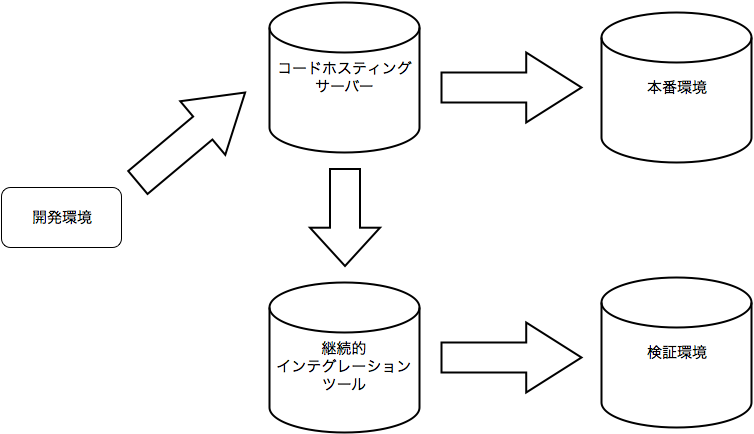
\includegraphics[height=8cm]{./assets/images/dev_env.png}
\caption{ソフトウェア開発の環境概要図}
\label{fig:dev_env}
\end{figure}

またそれらの環境構築する際に選定する必要のあるソフトウェアを列挙すると以下のようなものが挙げられる。

\begin{itemize}
 \item[・]プログラミング言語
   \begin{itemize}
    \item[・]アプリケーションフレームワーク
    \item[・]テスティングフレームワーク
    \item[・]アプリケーションサーバー
   \end{itemize}
 \item[・]バージョン管理システム
 \item[・]継続的インテグレーションシステム
 \item[・]OS
 \item[・]webサーバー
 \item[・]RDBMS
 \item[・]キャッシュサーバー
\end{itemize}

(レイヤーごとに分類する図が必要)

特に、プログラミング言語の選定は直下のレイヤーと、言語より上のレイヤーに影響を与える。どれを選ぶかは、既に言語を習得している人数や言語の習得難易度、言語を中心としたコミュニティやエコシステム\footnote{ライブラリの公開方法、インストールやアップデート、ライブラリ同士の依存関係の解決の仕組みなど、一つのソフトウェアを作る際に必要となる仕組みのつながり}が整備されているかに気を配らなければならない。またインターネットサービスを開発することに主眼を置くと、そのためのライブラリや共通規格が整備されているかも考慮する必要がある。その中でも、本論文執筆の時点で、考慮すべき点をクリアしており、企業での採用事例として出てくることが多いプログラミング言語のRubyの例をここで紹介し、それ以外の代表例はAppendixに記載する。

(レイヤーごとに分類する図 + Rubyでマッピングした図)
